% arara: pdflatex
% arara: bibtex
% arara: pdflatex
% arara: pdflatex

\documentclass{article}

% -----------------------------------------------------------------------------------------------------------------
% MACROS AND EXAMPLES OF WRITING SEMANTICS IN LaTeX 
% -----------------------------------------------------------------------------------------------------------------
	
	% -------------------------------------------------------------------------------------------------------------
	% PACKAGES NEEDED FOR WRITING LINGUISTICS SEMANTICS DENOTATION MACROS AND EXPLANATIONS
	% -------------------------------------------------------------------------------------------------------------
	
	\usepackage{stmaryrd} % used for the denotation brackets ('[[' and ']]'), which are part of this package and are written so as to be delimiters
	\usepackage{amsmath} % used to provide the \text command so that the text inside the denotation brackets is _not_ set in math mode 
	\usepackage{ragged2e} % used to provide the \RaggedRight command, which wraps text with both a ragged-right margin and hyphenation
	\usepackage{varwidth} % used to set the width of wrapped text to its natural width, lest the rightmost denotation bracket be offset based on the specified width

	% -------------------------------------------------------------------------------------------------------------
	% MACRO FOR THE INTERPRETATION FUNCTION
	% -------------------------------------------------------------------------------------------------------------
	
	\newcommand{\interp}[2][]{
	\(
		\left\llbracket\,\text{#2}\,\right\rrbracket^{#1}
	\)
	}

	% -------------------------------------------------------------------------------------------------------------
	% MACRO FOR WRAPPING LONG TEXT INSIDE DENOTATION
	% -------------------------------------------------------------------------------------------------------------
	
	\newcommand{\wraptext}[2][1in]{\begin{varwidth}{#1}{\RaggedRight#2}\end{varwidth}}
	
	% -------------------------------------------------------------------------------------------------------------
	% MACRO FOR LAMBDA EXPRESSIONS
	% -------------------------------------------------------------------------------------------------------------

	\newcommand{\lam}[2][]{$\lambda {#2}_{#1}$.}
	
	% -------------------------------------------------------------------------------------------------------------
	% MACRO FOR EXPLICIT LAMBDA EXPRESSIONS
	% -------------------------------------------------------------------------------------------------------------

	\newcommand{\lamexp}[2]{$\lambda {#1} \in D_{#2}$.}

	% -------------------------------------------------------------------------------------------------------------
	% MACRO FOR DENOTATION BRACKETS, TO BE USED WITH \WRAPTEXT
	% -------------------------------------------------------------------------------------------------------------

	\newcommand{\den}[1]{
	\(
		\left[\,\text{#1}\,\right]
	\)
	}

	% -------------------------------------------------------------------------------------------------------------
	% MACRO FOR ARGUMENT PARENTHESES, TO BE USED WITH \WRAPTEXT
	% -------------------------------------------------------------------------------------------------------------

	\newcommand{\argum}[1]{
	\(
		\left(\,\text{#1}\,\right)
	\)
	}

% -----------------------------------------------------------------------------------------------------------------
% END SEMANTICS MACROS
% -----------------------------------------------------------------------------------------------------------------

% -----------------------------------------------------------------------------------------------------------------
% BAD \WRAPTEXT COMMAND FOR ILLUSTRATION PURPOSES
% -----------------------------------------------------------------------------------------------------------------

\newcommand{\wraptextbad}[2][3in]{\parbox{#1}{\RaggedRight#2}}

% -----------------------------------------------------------------------------------------------------------------
% BAD \INTERP COMMAND FOR ILLUSTRATION PURPOSES
% -----------------------------------------------------------------------------------------------------------------

\newcommand{\interpbad}[2][]{$\llbracket$#2$\rrbracket^{#1}$}

% -----------------------------------------------------------------------------------------------------------------
% GENERAL PACKAGES AND OPTIONS FOR TYPSETTING THIS DOCUMENTATION FOR THE SEMANTICS MACROS
% -----------------------------------------------------------------------------------------------------------------

\usepackage{multicol}

\usepackage{xcolor}
\definecolor{darkred}{HTML}{B22613}

\usepackage[colorlinks]{hyperref}
\hypersetup{linkcolor=darkred,citecolor=gray,urlcolor=cyan}

\usepackage{natbib}
\setcitestyle{notesep={:}}

\usepackage{verbatim}
\usepackage{enumitem}
\usepackage{qtree}
\usepackage{tikz}
\usepackage{tikz-qtree,tikz-qtree-compat}
\tikzset{every tree node/.style={align=center, anchor=north}}
\usetikzlibrary{positioning,shapes,snakes}
\usepackage{fixltx2e}
\usepackage{gb4e}

\title{\texttt{lingsem} \\ Macros for Typesetting Semantics (Linguistics) \\ Version 0.1}
\author{Adam Liter}
\date{Last updated: \today}
\setcounter{section}{-1}

\begin{document}

\maketitle

\begin{abstract}
This document is documentation (pun intended) for \LaTeX\ macros that have been written in order to make the typesetting of semantics both easier and more readable. Section~\ref{sec:examples} includes explanations of how the macros work, using examples for illustration purposes. Section~\ref{sec:macros} provides definitions of the macros themselves. Section~\ref{sec:acknowledgements} includes some kudos to \href{http://tex.stackexchange.com/users/2693/alan-munn}{Alan Munn} for helping with these macros. And, finally, section~\ref{sec:changes} documents changes that have been made to these macros over time. 
\end{abstract}

\section{Introductory Remarks}

These are \LaTeX\ macros that aim to make the typesetting of work in semantics easier and the markup more readable. There is an unfortunate dearth of tools available to do so. Perhaps these macros will become a full-fledged package at some point. At the moment, however, the macros are rather skimpy and not, I think, worth putting on \href{http://ctan.org}{CTAN}.

That being said, any suggestions, comments, and improvements that \textbf{you} might have might lead to this becoming a more robust set of macros worth putting on \href{http://ctan.org}{CTAN}. If you do have suggestions, comments, or requests, please file them with the \href{https://github.com/adamliter/lingsem/issues}{GitHub issue tracker}. Or, if you want to contribute to development of these macros directly, fork \href{https://github.com/adamliter/lingsem}{the repo} and/or submit a pull request.

At any rate, the source code for these macros is documented below and examples of usage are interspersed throughout this documentation. The source code for the documentation and the source code for the macros themselves are available in the \href{https://github.com/adamliter/lingsem}{GitHub repo}.

\section{Examples \& Explanations}\label{sec:examples}

\subsection{The Interpretation Function}

There are two relevant macros for typesetting text inside of the semantic interpretation function (`$\llbracket$~$\rrbracket$'). They are \verb|\interp| and \verb|\wraptext|. \verb|\interp| takes an optional argument, which can be used to relativize the interpretation function to an assignment.\footnote{Assignment functions are used primarily to account for indexicals like pronouns \citep[\emph{e.g.},][90--95]{heim1998}. When doing intensional semantics, we might also want to relativize the interpretation function to a world of evaluation. The optional argument allows us to do so.} For example, \verb|\interp{fast}| produces the expression in (\ref{ex:no-assignment-function}), while \verb|\interp[g]{fast}| produces the expression in (\ref{ex:assignment-function}).

\textbf{Note} that the \verb|\interp| command is written so that the optional argument is in a math-mode environment. Thus, for example, if we want to relativize the interpretation function to a world of interpretation, say $w_{7}$, we write \verb|\interp[w_{7}]{fast}|---which produces the expression in (\ref{ex:world})---and \textbf{not} \verb|\interp[w$_{7}$]{fast}|, which will cause the compilation to crash.

\begin{exe}
	%
	\ex{
		%
		\begin{xlist}
			%
			\ex{\interp{fast}}\label{ex:no-assignment-function}
			%
			\ex{\interp[g]{fast}}\label{ex:assignment-function}
			%
			\ex{\interp[w_{7}]{fast}}\label{ex:world}
			%
		\end{xlist}
		%
	}
	%
\end{exe}

The second macro, \verb|\wraptext|, is used for handling denotations that we wish to specify that are lengthy. It exploits the fact that the two commands from the \href{http://ctan.org/pkg/stmaryrd}{\texttt{stmaryrd} package}---\verb|\llbracket| and \verb|\rrbracket|---are written so as to be delimiters. \verb|\wraptext| goes inside the \verb|\interp| command. It is written so that it's default optional argument value is `1in'. 

Thus, \verb|\interp{\wraptext{example of . . .}}| will produce the expression in (\ref{ex:long-den-1in}). 

Similarly, if we write, \verb|\interp{\wraptext[2in]{example of . . .}}|, that will produce the expression in (\ref{ex:long-den-2in}).

The definition of the \verb|\wraptext| command uses a varwidth environment, which is made available by the varwidth package. This environment sets the width of its contents to their natural width; thus, we need never worry about setting the width of the \verb|\wraptext| command such that the right denotation bracket is offset because of how the text wraps, as is the case in (\ref{ex:bad-wrap}).

\begin{exe}
	%
	\ex{
		%
		\begin{xlist}
			%
			\ex{\interp{\wraptext{example of really long text inside an interpretation function which will continue as long as we like}}}\label{ex:long-den-1in}
			%
			\ex{\interp{\wraptext[2in]{example of really long text inside an interpretation function which will continue as long as we like}}}\label{ex:long-den-2in}
			%
			\ex{\interp{\wraptextbad{example of really long text inside an interpretation function which will continue as long as we like}}}\label{ex:bad-wrap}
			%
		\end{xlist}
		%
	}
	%
\end{exe}

\subsection{Denotations \& Arguments}

By making minor adjustments to the \verb|\interp| command, we can define two new commands, \verb|\den| and \verb|\argum|, which do the exact same thing for denotations and arguments that \verb|\interp| does for text inside of the interpretation function.\footnote{Note that these new commands no longer take an optional argument, as one---as far as I am aware---never need specify another argument of a denotation or an argument like one often must specify an assignment function or world of evaluation for the interpretation function.} So, \verb|\den{x is fast in w}| produces the expression in (\ref{ex:denotation}). Similarly, \verb|\argum{Fred}| produces the expression in (\ref{ex:argument}). Both of these commands also work with the \verb|\wraptext| command just like \verb|\interp| does (\emph{cf}. (\ref{ex:denotation-wrap}) \& (\ref{ex:argument-wrap})).

\begin{exe}
	%
	\ex{
		%
		\begin{xlist}
			%
			\ex{\den{x is fast in w}}\label{ex:denotation}
			%
			\ex{\argum{Fred}}\label{ex:argument}
			%
			\ex{\den{\wraptext{example of a really long denotation which will continue as long as we like}}}\label{ex:denotation-wrap}
			%
			\ex{\argum{\wraptext{example of a really long argument which will continue as long as we like}}}\label{ex:argument-wrap}
			%
		\end{xlist}
		%
	}
	%
\end{exe}

\subsection{$\lambda$-expressions}

For lambda expressions, we can use one of two commands, either \verb|\lam| or \verb|\lamexp|. \verb|\lamexp| allows one to write a complete and explicit $\lambda$-expression as in (\ref{ex:lambda-full}). This command necessarily takes two arguments. Thus, to produce (\ref{ex:lambda-full}), we write \verb|\lamexp{p}{<s,t>}|.

\begin{exe}
	%
	\ex{
		%
		\begin{xlist}
			%
			\ex{\label{ex:lambda-full}\lamexp{p}{<s,t>}}
			%
			\ex{\label{ex:no-domain}\lam{p}}
			%
			\ex{\label{ex:yes-domain}\lam[<s,t>]{p}}
			%
		\end{xlist}
		%
	}
	%
\end{exe}

Often, though, we are satisfied with either of the abbreviations seen in (\ref{ex:no-domain}) or (\ref{ex:yes-domain}). We can produce either of these with the \verb|\lam| command. This macro takes an optional argument which can be used to specify the domain of the variable in the $\lambda$-expression. So, \verb|\lam{p}| produces the expression in (\ref{ex:no-domain}), and \verb|\lam[<s,t>]{p}| produces the expression in (\ref{ex:yes-domain}). 

Similar to the \verb|\interp| command, note that both the \verb|\lam| command and the \verb|\lamexp| are written so that all of their arguments are in a math-mode environment.

\subsection{Putting It All Together}

(\ref{ex:all}) is an example---abstracting away from many minor details---of how these commands can be used for readability's sake for computing the semantic derivation of the structure in (\ref{ex:all-tree}), whereas (\ref{ex:all-bad}) is an example of what (\ref{ex:all}) might look like without these macros.

\begin{exe}
	%
	\ex{
		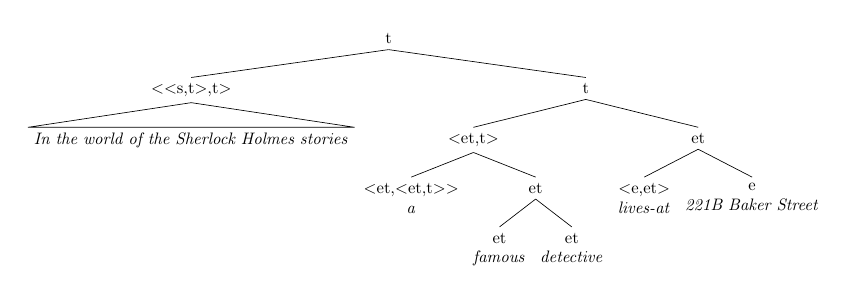
\begin{tikzpicture}[scale=.6,baseline]
			\Tree
			[.t
				[.$<<$s,t$>$,t$>$ \edge[roof]; {\textit{In the world of the Sherlock Holmes stories}} ]
				[.t
					[.$<$et,t$>$
						[.$<$et,$<$et,t$>>$\\\textit{a} ]
						[.et
							[.et\\\textit{famous} ]
							[.et\\\textit{detective} ]
						]
					]
					[.et
						[.$<$e,et$>$\\\textit{lives-at} ]
						[.e\\\textit{221B Baker Street} ]
					]
				]
			]
		\end{tikzpicture}
	}\label{ex:all-tree}
	%
	\ex{
		%
		\begin{xlist}
			%	
			\ex{\interp[w_{7},g]{\wraptext{a famous detective lives at 221B Baker Street}} = \wraptext[2.5in]{1 iff $\exists$x : x is famous in w$_{7}$ and x is a detective in w$_{7}$ and x lives at 221B Baker Street in w$_{7}$}
			\\
			\\
			}
			%
			\ex{\interp[w_{7},g]{\wraptext[0.8in]{In the world of the Sherlock Holmes stories, a famous detective lives at 221B Baker Street}} = \interp[w_{7},g]{\wraptext[0.7in]{In the world of the Sherlock Holmes stories}}\argum{\wraptext[1.6in]{\wraptext[1.3in]{\lam{w}~\interp[w,g]{\wraptext[0.6in]{a famous detective lives at 221B Baker Street}}}}
			\\
			\\}
			\\
			\\ = \den{\wraptext{$\forall$w$'$ compatible with the Sherlock Holmes stories in w, p(w$'$) = 1}}\argum{\wraptext[1.7in]{\lam{w}~\interp[w,g]{\wraptext{a famous detective lives at 221B Baker Street}}}}
			\\
			\\
			\\ = \wraptext[3.5in]{1 iff, $\forall$w$'$ compatible with the Sherlock Holmes stories in w, $\exists$x : x is famous in w$'$ and x is a detective in w$'$ and x lives at 221B Baker Street in w$'$}
			\\
			}
			%
		\end{xlist}
		%	
	}\label{ex:all}
	%
	\ex{
		%
		\begin{xlist}
			%
			\ex{\interpbad[w_{7},g]{a famous detective lives at 221B Baker Street} = 1 iff $\exists$x : x is famous in w$_{7}$ and x is a detective in w$_{7}$ and x lives at 221B Baker Street in w$_{7}$
			\\
			}
			%
			\ex{\interpbad[w_{7},g]{In the world of the Sherlock Holmes stories, a famous detective lives at 221B Baker Street} = \interpbad[w_{7},g]{In the world of the Sherlock Holmes stories}(\lam{w}\interpbad[w,g]{a famous detective lives at 221B Baker Street})
			\\
			\\ = [$\forall$w$'$ compatible with the Sherlock Holmes stories in w, p(w$'$) = 1](\lam{w}\interpbad[w,g]{a famous detective lives at 221B Baker Street})
			\\
			\\ = 1 iff, $\forall$w$'$ compatible with the Sherlock Holmes stories in w, $\exists$x : x is famous in w$'$ and x is a detective in w$'$ and x lives at 221B Baker Street in w$'$
			}
			%
		\end{xlist}
		%
	}\label{ex:all-bad}
	%
\end{exe}

In my opinion, at least, the version in (\ref{ex:all}) looks much better and is much more readable than the version in (\ref{ex:all-bad}).

\section{\label{sec:macros}Writing the Macros}

\subsection{Writing the Macros Yourself}

If you would like, you can follow the instructions below to write the macros yourself.

\subsubsection{Required Packages}

In order to write these macros, you will need to load the following packages in your \texttt{.tex} document.

\begin{multicols}{2}
\begin{itemize}

	\item{\href{http://ctan.org/pkg/stmaryrd}{\texttt{stmaryrd}}}
	
	\item{\href{http://ctan.org/pkg/amsmath}{\texttt{amsmath}}}
	
	\item{\href{http://ctan.org/pkg/ragged2e}{\texttt{ragged2e}}}
	
	\item{\href{http://ctan.org/pkg/varwidth}{\texttt{varwidth}}}

\end{itemize}
\end{multicols}

\subsubsection{The Macros}

In order to use the macros, define the following commands in the preamble of your \texttt{.tex} document.

\begin{itemize}

	\item{\verb|\interp| is defined as follows:
	\begin{verbatim}
	\newcommand{\interp}[2][]{
	\(
		\left\llbracket\,\text{#2}\,\right\rrbracket^{#1}
	\)
	}
	\end{verbatim}
	}
	
	\item{\verb|\den| is defined as follows:
	\begin{verbatim}
	\newcommand{\den}[1]{
	\(
		\left[\,\text{#1}\,\right]
	\)
	}
	\end{verbatim}
	}
	
	\item{\verb|\argum| is defined as follows:
	\begin{verbatim}
	\newcommand{\argum}[1]{
	\(
		\left(\,\text{#1}\,\right)
	\)
	}
	\end{verbatim}
	}
	
	\item{\verb|\wraptext| is defined as follows:
	\begin{verbatim}
	\newcommand{\wraptext}[2][1in]{
	\begin{varwidth}{#1}{\RaggedRight#2}\end{varwidth}
	}
	\end{verbatim}
	}
	
	\item{\verb|\lam| is defined as follows:
	\begin{verbatim}
	\newcommand{\lam}[2][]{$\lambda {#2}_{#1}$.}
	\end{verbatim}
	}
	
	\item{\verb|\lamexp| is defined as follows:
	\begin{verbatim}
	\newcommand{\lamexp}[2]{$\lambda {#1} \in D_{#2}$.}
	\end{verbatim}
	}	

\end{itemize}

\subsection{Downloading the Macros}

If you would rather not write the macros yourselves, you can simply download the source code directly for these macros from the \href{https://github.com/adamliter/lingsem}{GitHub repo} and place them in your preamble.

Or, if you use TeXShop, this \texttt{.tex} file can then be placed in the Templates directory (\verb|~/Library/TeXShop/Templates|), which will allow you to access the macros from the Templates menu in TeXShop.

\section{\label{sec:acknowledgements}Acknowledgements}

The two macros, \verb|\interp| \& \verb|\wraptext|, were written by \href{http://tex.stackexchange.com/users/2693/alan-munn}{Alan Munn} in response to a question that I posted on \href{http://tex.stackexchange.com/questions/121605/macro-for-typesetting-semantic-denotations-linguistics}{TeX.SX}. I adapted the \verb|\den| and \verb|\argum| commands from his macro for \verb|\interp|, and I wrote the two macros for $\lambda$-expressions myself.

\section{\label{sec:changes}Change Log}

\begin{description}

\item[Version 0.1 (2014.06.02)]{Pushed the macros to GitHub.}

\end{description}

\bibliographystyle{unified} % This bib style is available here: http://celxj.org/downloads/unified.bst
\bibliography{lingsem}

\end{document}